\documentclass[nobib]{tufte-handout}

\title{Lecture 14: The probabilistic method and the Erd\H{o}s-Rényi random graph $\cdot$ 1MA170}

\author[Vilhelm Agdur]{Vilhelm Agdur\thanks{\href{mailto:vilhelm.agdur@math.uu.se}{\nolinkurl{vilhelm.agdur@math.uu.se}}}}

\date{28 November 2023}


%\geometry{showframe} % display margins for debugging page layout

\usepackage{graphicx} % allow embedded images
  \setkeys{Gin}{width=\linewidth,totalheight=\textheight,keepaspectratio}
  \graphicspath{{graphics/}} % set of paths to search for images
\usepackage{amsmath}  % extended mathematics
\usepackage{booktabs} % book-quality tables
\usepackage{units}    % non-stacked fractions and better unit spacing
\usepackage{multicol} % multiple column layout facilities
\usepackage{lipsum}   % filler text
\usepackage{fancyvrb} % extended verbatim environments
  \fvset{fontsize=\normalsize}% default font size for fancy-verbatim environments

\usepackage{color,soul} % Highlights for text

% Standardize command font styles and environments
\newcommand{\doccmd}[1]{\texttt{\textbackslash#1}}% command name -- adds backslash automatically
\newcommand{\docopt}[1]{\ensuremath{\langle}\textrm{\textit{#1}}\ensuremath{\rangle}}% optional command argument
\newcommand{\docarg}[1]{\textrm{\textit{#1}}}% (required) command argument
\newcommand{\docenv}[1]{\textsf{#1}}% environment name
\newcommand{\docpkg}[1]{\texttt{#1}}% package name
\newcommand{\doccls}[1]{\texttt{#1}}% document class name
\newcommand{\docclsopt}[1]{\texttt{#1}}% document class option name
\newenvironment{docspec}{\begin{quote}\noindent}{\end{quote}}% command specification environment

\include{mathcommands.extratex}

\begin{document}

\maketitle% this prints the handout title, author, and date

\begin{abstract}
\noindent
We introduce a new tool to the course, the probabilistic method, and use it to prove some new results. We also introduce the Erd\H{o}s-Rényi random graph, which is interesting in its own right as well as being a tool in the probabilistic method.
\end{abstract}

\section{The minimum bisection problem}

Suppose we are given a graph $G$, which is too large to fit on a single computer -- so we wish to distribute the computation we want to do on the graph between two machines. We imagine the computation we want to do is in some sense possible to do ``locally'' -- so if the graph had two equally sized connected components, the two computers wouldn't have to talk to each other at all.

Of course, most graphs do not split up that nicely, but we can still try to divide it into two equally sized parts that have as few edges between them as possible. How well can we do this?

\begin{proposition}
  For any graph $G = (V,E)$ on $n \in 2\N$ vertices with maximum degree $\Delta < \frac{n}{2}$, there exists a partition $A \coprod B$ of $V$, such that $\abs{A} = \abs{B} = \frac{n}{2}$, and
  $$e(A,B) \leq \frac{\abs{E}}{2},$$
  where $e(A,B)$ is the number of edges between $A$ and $B$.

  \begin{proof}
    Let $G^c$ be the complement graph of $G$ -- that is, $G^c$ has the same vertices as $G$, and there is an edge $x \sim y$ in $G^c$ if and only if $x \sim y$ is not an edge of $G$.

    Since we assumed $\Delta < \frac{n}{2}$, it is clear that the \emph{minimum} degree of $G^c$ is at least $\frac{n}{2}$, and so by Dirac's theorem\sidenote[][]{Which we proved earlier in the course.} there exists a Hamilton cycle in $G^c$. Picking every second edge of this Hamilton cycle, we get a perfect matching $M$ on $G^c$. This process is illustrated in Figure~\ref{fig:min_bisection_matching}.

    \begin{figure}
      \centering
      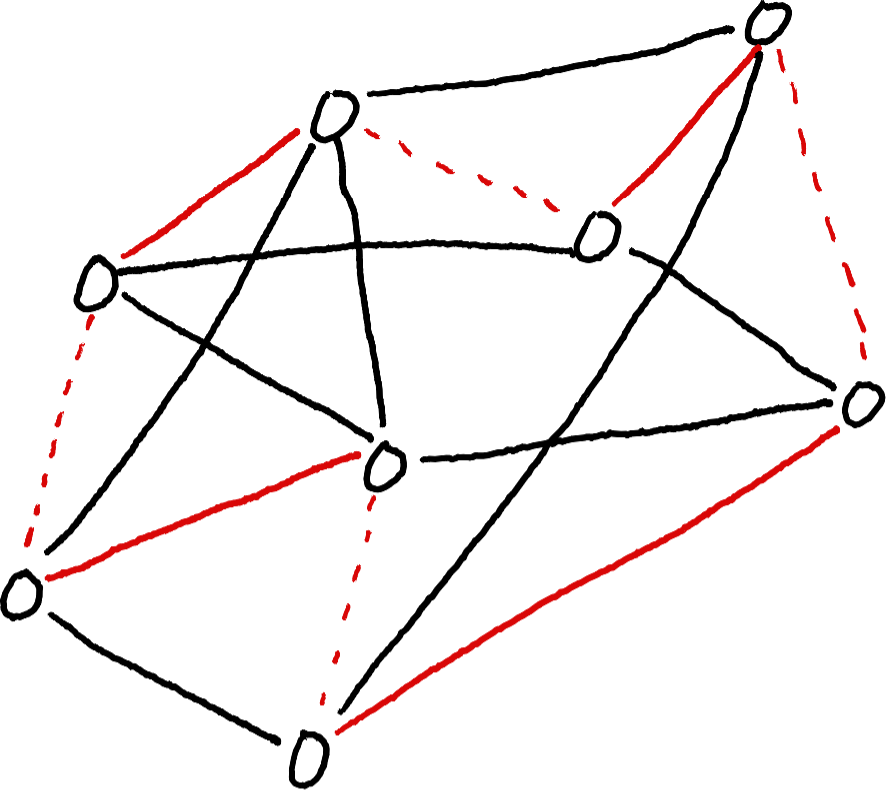
\includegraphics[width=0.7\textwidth]{L14_probabilistic_method/min_bisection_matching.png}
      \caption{A graph on eight vertices, with its edges drawn in black. Since it has maximum degree three, we can find a Hamilton cycle in its complement graph, which has been drawn with alternating dotted and stroked red lines. By picking only the stroked red lines, we get a perfect matching in the complement of the graph.}
      \label{fig:min_bisection_matching}
    \end{figure}

    Now, we apply the probabilistic method, picking a random partition $A \coprod B$ of $V$: For each edge of $M$, we randomly place one of its endpoints in $A$ and one in $B$, independently between different edges. We can then compute that
    \begin{align*}
      \E{\abs{e(A,B)}} &= \E{\sum_{x \sim y \in E} \ind{x \sim y \in E(A,B)}}\\
      &= \sum_{x \sim y \in E} \Prob{x\text{ and }y\text{ are in different sets}}.
    \end{align*}

    Now, whenever $x$ and $y$ are not connected by an edge in $M$, their assignment to $A$ or $B$ is independent, and so the probability that they are in different sets is precisely $\frac{1}{2}$. However, we picked our matching $M$ so that it is a perfect matching on $G^c$ -- in particular this means that $M \cap E = \emptyset$, and so all of the probabilities that we are summing must in fact be $\frac{1}{2}$ by our previous argument.

    So the sum is just a sum of $\abs{E}$ many $\frac{1}{2}$'s, and so what we have seen is that $\E{\abs{e(A,B)}} = \frac{\abs{E}}{2}$. Now, we know that the expectation is never greater than every specific outcome, so there must exist some choice of $A$ and $B$ with no more than $\frac{\abs{E}}{2}$ edges between them, and we have shown the proposition.
  \end{proof}
\end{proposition}

\section{The Erd\H{o}s-Rényi graph}

As we saw in the previous exercise session, the simplest and most common random graph model is the Erd\H{o}s-Rényi graph, where all edges appear independently with the same probability. Let us restate the definition here, for completeness.

\begin{definition}
  For any integer $n \in \N$ and any probability $p \in [0,1]$, the \emph{Erd\H{o}s-Rényi graph} $G(n,p)$ is a random graph on $n$ vertices,\sidenote[][]{We will normally assume its vertex set is $[n]$, unless otherwise stated.} where each of the $\binom{n}{2}$ potential edges is present independently at random with probability $p$.
\end{definition}

\begin{proposition}
  Let $\Hat G = (V,E)$ be a labelled graph on $n$ vertices, and $G = G(n,p)$ be an Erd\H{o}s-Rényi graph on the same number of vertices. The probability that $G = \Hat G$ is precisely
  $$\Prob{G = \Hat G} = p^{\abs{E}}(1-p)^{\binom{n}{2} - \abs{E}},$$
  and so in particular if $p = \frac{1}{2}$, the Erd\H{o}s-Rényi graph is in fact a uniformly random graph.
\end{proposition}

We proved two things about the Erd\H{o}s-Rényi graph during the exercises, but let us restate those results and their proofs here.

\begin{lemma}\label{lemma:er_independence_number}
  If $G = G(n,p)$ is an Erd\H{o}s-Rényi graph, the probability that it has an independent set of size at least $k$ is bounded by
  $$\Prob{\alpha(G) \geq k} \leq \binom{n}{k}(1-p)^{\binom{k}{2}}.$$

  \begin{proof}
    There are a total of $\binom{n}{k}$ subsets of $[n]$ of size $k$, so for each such set $X \in \binom{[n]}{k}$, let $A_X$ be the event that $X$ is an independent set in $G$.

    Clearly, $A_X$ happens whenever none of the $\binom{k}{2}$ possible edges inside $X$ are present, which happens with probability $(1-p)^{\binom{k}{2}}$. So we can calculate, using a union bound, that
    \begin{align*}
      \Prob{\alpha(G) \geq k} &= \Prob{\bigcup_{X \in \binom{[n]}{k}} A_X}\\
      &\leq \sum_{X \in \binom{[n]}{k}} \Prob{A_X}\\
      &= \sum_{X \in \binom{[n]}{k}} (1-p)^{\binom{k}{2}} = \binom{n}{k}(1-p)^{\binom{k}{2}}
    \end{align*}
    where we used in the last equality that we had $\binom{n}{k}$ summands, giving the lemma.
  \end{proof}
\end{lemma}

\begin{proposition}
  For any $p \in (0,1)$, if $G_n = G(n,p)$ is an Erd\H{o}s-Rényi graph for each $n$, it holds that
  $$\Prob{\diam(G_n) = 2} \to 1\quad\text{as}\quad n \to \infty.$$
\end{proposition}

It is somewhat cumbersome to explicitly write out the sequence of random graphs and the limit every time we want to say something about an asymptotic property of the Erd\H{o}s-Rényi graph, so we will generally use the following way of phrasing such results instead:

\begin{proposition}
  For each fixed $p \in (0,1)$, it holds that $\diam(G(n,p)) = 2$ with high probability.\sidenote[][-1cm]{We also synonymously say that a property holds ``asymptotically almost surely'' -- these two phrases are then abbreviated to ``w.h.p.'' or ``a.a.s.'' when convenient. In both cases, what we mean is that the property holds with probability tending to one as we increase the number of vertices of the graph.}

  \begin{proof}
    The only graphs with diameter one are the complete graphs, and it is easy to see\sidenote[][]{
      \begin{xca}
        See this.
      \end{xca}
    } that the Erd\H{o}s-Rényi graph is not complete w.h.p. for any $p < 1$. So all we need to do is to show that $\diam G(n,p) \leq 2$ w.h.p.

    So, for any pair of two distinct vertices $i$ and $j$, let $B_{ij}$ be the event that there is no edge between $i$ and $j$ and they additionally have no common neighbour. We call such a pair of vertices a \emph{bad} pair -- it is clear that a graph has diameter at most two precisely when it has no bad pairs.
    
    Now we can compute, using the fact that edges appear independently, that
    \begin{align*}
      \Prob{B_{ij}} &= \Prob{\left(i \sim j \not\in E\right) \wedge \left(\bigwedge_{k \in [n]\setminus \{i,j\}} (i \sim k \not\in E)\vee (k \sim j \not \in E)\right)}\\
      &= (1-p)\prod_{k \in [n] \setminus \{i,j\}} \Prob{(i \sim k \not\in E)\vee (k \sim j \not \in E)}\\
      &= (1-p)\prod_{k \in [n] \setminus \{i,j\}} (1 - p^2) = (1-p)(1 - p^2)^{n-2},
    \end{align*}
    and so letting $X$ be the number of bad pairs, we compute using linearity of expectation that
    \begin{align*}
      \E{X} &= \E{\sum_{\{i,j\} \in \binom{[n]}{2}} \ind{B_{ij}}}\\
      &= \sum_{\{i,j\} \in \binom{[n]}{2}} \Prob{B_{ij}}\\
      &= \binom{n}{2}(1-p)(1 - p^2)^{n-2}
    \end{align*}
    which we easily see goes to zero for fixed $p \in (0,1)$ as $n \to \infty$.

    The result now follows by following the recipe for the first-moment method, applying Markov's inequality to see that we also have $\Prob{X > 0} \to 0$ as $n \to \infty$.
  \end{proof}
\end{proposition}

\section{Triangles in the Erd\H{o}s-Rényi graph}

Having seen these two results from the exercises, let us do a slightly more involved calculation, that will make use of the second-moment method. In order to see interesting things happening in the $G(n,p)$, we will almost always have to choose a probability $p$ that shrinks as $n$ grows, to control the sparsity of the graph.

\begin{proposition}
  If $p = o\left(n^{-1}\right)$, $G(n,p)$ a.a.s. contains no triangle. If $p = \omega\left(n^{-1}\right)$, $G(n,p)$ contains a triangle w.h.p.\sidenote[][]{As a recap on the $O$ and $\Omega$ family of notations, recall that $f = o(g)$ means that $\lim_{n\to\infty} \frac{f(n)}{g(n)} = 0$, while $f = \omega(g)$ means that $\lim_{n\to\infty} \frac{f(n)}{g(n)} = \infty$.
  
  We will also use the notations $f \sim g$, which means that $\lim_{n\to\infty} \frac{f(n)}{g(n)} = 1$, and $f = O(g)$, which means that $f$ is asymptotically not of higher order than $g$, i.e. $\limsup_{n\to \infty} \frac{f(n)}{g(n)} < \infty$.
  
  Finally, we use the notation $f = \Theta(g)$, which means that $f = O(g)$ and $g = O(f)$, and use the fact that $f \sim g$ implies $f = \Theta(g)$ without comment.}

  \begin{proof}
    For each set $\tau$ of three vertices of $G$, i.e. three integers from $[n]$, let $T_\tau$ be the event that they form a triangle, and for convenience let us write $Y_\tau = \ind{T_\tau}$ for the indicator variable of this event. It is clear that $\Prob{T_\tau} = \E{Y_\tau} = p^3$, and so if we let the total number of triangles in $G$ be $X$, we compute by linearity of expectation that
    $$\E{X} = \E{\sum_{\tau \in \binom{[n]}{3}} Y_\tau} = \sum_{\tau \in \binom{[n]}{3}} \Prob{T_\tau} = \binom{n}{3}p^3 \sim (np)^3$$
    and so if $np \to 0$, we have $\E{X} \to 0$, and so by a first-moment method argument there are w.h.p. no triangles in $G$.

    Now, to prove that there are triangles if $p = \omega\left( n^{-1} \right)$, it does not suffice to see that the expected number of triangles is high,\sidenote[][]{As we discussed in the exercise sheet about this -- see them for an explanation of this.} and so we need to also compute the variance in the number of triangles.

    So we find that
    \begin{align*}
      \E{X^2} &= \E{\left(\sum_{\tau \in \binom{[n]}{3}} Y_\tau\right)^2}
      = \E{\sum_{\tau, \sigma \in \binom{[n]}{3}} Y_\tau Y_\sigma}\\
      &= \E{\sum_{\tau \in \binom{[n]}{3}} Y_\tau^2 + \sum_{\substack{\tau, \sigma \in \binom{[n]}{3}\\\tau \neq \sigma}} Y_\tau Y_\sigma}\\
      &= \sum_{\tau \in \binom{[n]}{3}} \E{Y_\tau^2} + \sum_{\substack{\tau, \sigma \in \binom{[n]}{3}\\\tau \neq \sigma}} \E{Y_\tau Y_\sigma},
    \end{align*}
    and for the first of the two sums we can notice that $Y_\tau = Y_\tau^2$ always, since it is always either zero or one, so that sum is in fact just $\E{X}$, and so we have seen that
    $$\E{X^2} = \E{X} + \sum_{\substack{\tau, \sigma \in \binom{[n]}{3}\\\tau \neq \sigma}} \E{Y_\tau Y_\sigma}.$$

    For the second term, we need to break it apart into how the two sets $\sigma$ and $\tau$ can overlap,\sidenote[][]{So far, this calculation has been in a sense ``entirely standard'' -- any second-moment method argument will involve these steps, up to looking at how the things we count can overlap. The points where they differ is just in how hard it is to understand these overlaps -- fortunately, how two triangles can overlap without being equal is pretty easy to see.} and so we write that
    \begin{align*}
      \sum_{\substack{\tau, \sigma \in \binom{[n]}{3}\\\tau \neq \sigma}} \E{Y_\tau Y_\sigma} &= \sum_{\substack{\tau, \sigma \in \binom{[n]}{3}\\\tau \cap \sigma = \emptyset}} \E{Y_\tau Y_\sigma} + \sum_{\substack{\tau, \sigma \in \binom{[n]}{3}\\\abs{\tau \cap \sigma = 1}}} \E{Y_\tau Y_\sigma} + \sum_{\substack{\tau, \sigma \in \binom{[n]}{3}\\\abs{\tau \cap \sigma} = 2}} \E{Y_\tau Y_\sigma}
    \end{align*}
    and analyse each case separately.

    If they do not overlap at all, then there are six edges that need to be present, and so $\E{Y_\tau Y_\sigma} = p^6$. There are $\binom{n}{3}\binom{n-3}{3}$ ways to choose two disjoint sets of size three, and so in total\sidenote[][]{We choose not to summarize this term with a big-O because we will need to compare it to a different thing of the same order later, so we do need the exact value. For the rest of the terms, we summarize them, since we don't need more details.}
    $$\sum_{\substack{\tau, \sigma \in \binom{[n]}{3}\\\tau \cap \sigma = \emptyset}} \E{Y_\tau Y_\sigma} = p^6\binom{n}{3}\binom{n-3}{3}$$% = O\left((pn)^6\right).$$

    If they overlap in a single vertex, there are still six edges that need to be present, so we still have $\E{Y_\tau Y_\sigma} = p^6$. However, there are $n\binom{n-1}{2}\binom{n-3}{2}$ ways to choose two sets of size three that overlap in one vertex, and so we see that
    $$\sum_{\substack{\tau, \sigma \in \binom{[n]}{3}\\\abs{\tau \cap \sigma = 1}}} \E{Y_\tau Y_\sigma} = p^6 n\binom{n-1}{2}\binom{n-3}{2} = O\left(p^6 n^5\right).$$

    Finally, if they overlap in two vertices, there are only five edges that need to be present, and so we now have $\E{Y_\tau Y_\sigma} = p^5$. There are $\binom{n}{2}(n-2)(n-3)$ ways to choose two sets of size three that overlap in two vertices, and so we have
    $$\sum_{\substack{\tau, \sigma \in \binom{[n]}{3}\\\abs{\tau \cap \sigma = 2}}} \E{Y_\tau Y_\sigma} = p^5 \binom{n}{2}(n-2)(n-3) = O\left(p^5 n^4\right).$$

    Assembling this calculation, we find that
    \begin{align*}
      \E{X^2} &= \E{X} + p^6\binom{n}{3}\binom{n-3}{3} + O\left(p^6 n^5\right) + O\left(p^5 n^4\right)\\
      &= O\left(p^3 n^3\right) + p^6\binom{n}{3}\binom{n-3}{3} + O\left(p^6 n^5\right) + O\left(p^5 n^4\right)
    \end{align*}
    and so
    \begin{align*}
      \Var{X} &= \E{X^2} - \E{X}^2\\
      &= O\left(p^3 n^3\right) + p^6\binom{n}{3}\binom{n-3}{3} + O\left(p^6 n^5\right) + O\left(p^5 n^4\right) - \left(\binom{n}{3} p^3\right)^2\\
      &\leq O\left(p^3 n^3\right) + O\left(p^6 n^5\right) + O\left(p^5 n^4\right)
    \end{align*}
    where we did a somewhat messy calculation to get the final inequality.\sidenote[][]{In particular, we observe that
    $$\binom{n}{3}\binom{n-3}{3} - \left(\binom{n}{3} p^3\right)^2$$
    equals
    $$-\frac{1}{12} n (3 n^4 - 24 n^3 + 71 n^2 - 90 n + 40)$$
    and so it is asymptotically negative, and so we get the inequality when we drop both terms.}

    So if we follow the recipe we gave in the exercises for the second-moment method, we now need to compare the variance to $\E{X}^2$, which we do, seeing that
    \begin{align*}
      \frac{\Var{X}}{\E{X}^2} &\leq \frac{O\left(p^3 n^3\right) + O\left(p^6 n^5\right) + O\left(p^5 n^4\right)}{\left(\Theta\left(n^3 p^3\right)\right)^2}\\
      &= O\left((pn)^{-3}\right) + O\left(n^{-1}\right) + O\left((pn)^{-1}n^{-1}\right)
    \end{align*}
    which we see must go to zero with $n$ if $pn \to \infty$ with $n$. Thus our lemma for the second-moment method gives us that
    $$\Prob{X = 0} \leq \frac{\Var{X}}{\E{X}^2} \to 0,$$
    and so $G$ contains at least one triangle, as desired.
  \end{proof}
\end{proposition}

\section{The growth of $G(n,p)$}

We have seen whether $G(n,p)$ contains triangles if $p$ is asymptotically less than or greater than $\frac{1}{n}$. What happens if $p = \frac{c}{n}$ for some $c>0$? This turns out to be the ``critical'' range for a lot of interesting questions. In this case, a $G\left(n, \frac{c}{n}\right)$ will contain a Poisson distributed amount of triangles, with mean $\frac{c^3}{6}$ -- so sometimes it has a triangle and sometimes it does not!

Let us sketch a few more things that can be said about how the structure of $G(n,p)$ changes as the value of $p$ changes. Many more things can be said, but since we aren't going to prove any of them, we just give an outline here.

\begin{itemize}
  \item If $p = o\left(n^{-1}\right)$ we don't just get no triangles, we in fact get no cycles of any length -- so $G(n,p)$ is a forest.
  \item For $p = \frac{c}{n}$ with $0 < c < 1$, each connected component is either a tree or contains a single cycle. If $C_{\max}$ denotes the number of vertices in the largest component, we have
  $$\frac{C_{\max}}{\log(n)} \to \frac{1}{c - 1 - \log(c)}$$
  in probability.\sidenote[][]{A sequence of random variables $X_n$ converges to $a \in \R$ \emph{in probability} if, for every $\epsilon > 0$,
  $$\Prob{\abs{X_n - a} > \epsilon} \to 0$$
  as $n \to \infty$. Note the order of the quantifiers here: This is a pointwise thing, in that we first fix $\epsilon$ and then take the limit. It is not equivalent to ask that this thing go to zero for every $\epsilon$ simultaneously.}
  \item If $p = \frac{1}{n}$ exactly, the largest component has about $n^{2/3}$ vertices.
  \item For every $c > 1$ there exists a constant $\zeta_c > 0$ such that the largest connected component of $G\left(n, \frac{c}{n}\right)$ contains about a $\zeta_c$ fraction of the vertices, up to an error of about $\pm \sqrt{n}$.\sidenote[][]{Here is an incredibly precise version of this statement, for those of you who really enjoy quantifiers and constants:
  
  \begin{align*}
    \forall c > &1 \,\exists \zeta_c > 0\, \forall \nu \in \left(\frac{1}{2},1\right) \exists \delta > 0:\\ &\Prob{\abs{C_{\max} - \zeta_c n} \geq n^\nu} = O\left(n^{-\delta}\right).
  \end{align*}}

  This largest component is unique, and is called the \emph{giant component} -- all other connected components are trees on $O\left(\log(n)\right)$ vertices. The giant component contains enough edges to be non-planar.
  \item If $p = c\frac{\log(n)}{n}$, the graph is a.a.s. connected and Hamiltonian.
\end{itemize}

\section{Girth and chromatic number}

Already when we first introduced the chromatic number, we mentioned the obvious fact that a large clique forces a graph to have high chromatic number. One might be led by this to believe that being very sparse, without any cliques, would mean you have low chromatic number. This unfortunately turns out to be not at all true, in a pretty strong sense.

\begin{definition}
  The \emph{girth} of a graph $G$ is the length of the shortest cycle in the graph.
\end{definition}

So the notion of girth generalizes the notion of being triangle-free, which is just having girth greater than three. Of course any triangle-free graph also contains no larger cliques, so this is indeed a strong notion of having no cliques.

\begin{theorem}[Erd\H{o}s, 1959]\label{thm:high_girth_high_chromatic_number}
  For all positive integers $k$ there exists a graph $G$ of girth and chromatic number at least $k$.
\end{theorem}

We leave the full proof as an exercise, but let us give a sketch of how it is done in the lecture itself.

\begin{proof}[Proof sketch]
  Fix a $k \geq 3$ and an $\epsilon \in \left(0, \frac{1}{k}\right)$, and let $p = n^{-(1-\epsilon)}$. Let $G$ be a $G(n,p)$. Our strategy is the following:
  \begin{enumerate}
    \item We count the number of cycles of length at most $k$ in $G$, and show that with probability greater than $\frac{1}{2}$ there are fewer than $\frac{n}{2}$ of them.
    \item We calculate the probability that $G$ has no independent set of size $\frac{n}{2k}$, and see that this is greater than $\frac{1}{2}$.
    \item We observe that two events both of which have probability greater than one half cannot be disjoint, so there exists some graph $\Hat G$ which has fewer than $\frac{n}{2}$ cycles of length at most $k$ and has independence number less than $\frac{n}{2k}$.
    \item We finally observe that if we remove one vertex from each cycle of $\Hat G$ we get an induced subgraph $H$ with girth at least $k$ and independence number at most $\frac{n}{2k}$, and so we can apply the inequality
    $$\chi(H) \geq \frac{\abs{V(H)}}{\alpha(H)}$$
    to get that the chromatic number of $H$ is also at least $k$. So $H$ is a graph of the type we desired to show exists.
  \end{enumerate}
\end{proof}

\section{Exercises}

\begin{xca}
  In this exercise, we will implement the proof sketch for Theorem \ref{thm:high_girth_high_chromatic_number} -- so take $G$ as we did there, and then:

  \begin{enumerate}[label=\alph*)]
    \item Letting $X_i$ be the number of cycles of length $i$ in $G$, show that
    $$\E{X_i} = \frac{n!}{(n-i)!}\frac{p^i}{2i}.$$
    \item Now let $X = \sum_{i=3}^k X_i$, and use the above to show that
    $$\E{X} \leq \frac{1}{2}(k-2)(np)^k.$$
    \item Use Markov's inequality to show that $\Prob{X \geq \frac{n}{2}} \to 0$ with $n$, and conclude that $G$ a.a.s. has less than $\frac{n}{2}$ cycles of length at most $k$.
    \item Modify the proof of Lemma \ref{lemma:er_independence_number} to see that
    $$\Prob{\alpha(G) \geq \frac{n}{2k}} \to 0 \quad \text{as} \quad n \to \infty$$
    whenever $p \geq \frac{16k^2}{n}$ for all sufficiently large $n$.
    \item Conclude that for sufficiently large $n$,
    $$\Prob{X < \frac{n}{2}} > \frac{1}{2}\quad\text{and}\quad\Prob{\alpha(G) < \frac{n}{2k}} > \frac{1}{2},$$
    and thus the events cannot be disjoint, and there must exist a graph $\Hat G$ with both these properties.
    \item Consider an induced subgraph $H$ of $\Hat G$ gotten by removing one vertex from each cycle of length at most $k$ in $\Hat G$. Show that $\abs{V(H)} \geq \frac{n}{2}$, the girth of $H$ is at least $k$, and $\alpha(H) \leq \alpha(\Hat G)$.
    \item Use the inequality $\chi(H) \geq \frac{\abs{V(H)}}{\alpha(H)}$ and what you just saw in the previous step to conclude that $\chi(H) \geq k$, yielding the theorem.
  \end{enumerate}
\end{xca}


%\bibliography{references}
%\bibliographystyle{plainnat}

\end{document}
